In this chapter, the theoretical background necessary to the understanding and simulation of a hyperfine spectrum is presented. $\S$ \ref{AHF} describes how the features of a hyperfine spectrum are linked to physical properties of a nucleus, while $\S$ \ref{ALI} outlines the way in which lasers interact with atoms.
Note: Throughout this section, a variable written in a bold typeface is vector valued, while its non-bold counterpart is its magnitude. 
\section{Anatomy of a Hyperfine Spectrum}
\label{AHF}
\begin{figure}[h]
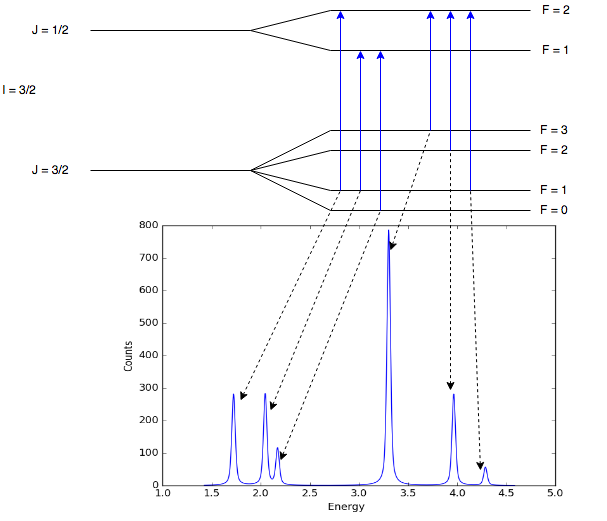
\includegraphics[width=\textwidth]{Graphics/spec_with_peaks_4.png}
\caption[Hyperfine spectrum and level-scheme for Gallium-69.]{Hyperfine spectrum and level-scheme for the 4P$_{3/2}\rightarrow$5S$_{1/2}$ transition in atomic Gallium-69. Photon counts are shown on the vertical axis, while the horizontal shows the energies of the photons. Each allowed transition in the level-scheme is linked to the relevant peak in the hyperfine spectrum.}
\label{ga69}
\end{figure}
How can the properties of a hyperfine spectrum, such as that of $^{69}\mathrm{Ga}$ shown in Fig.\ref{ga69}, be translated into measurements of the physical properties of the nucleus? The hyperfine spectrum is, after all, the result of probing the electronic structure of the atom. The answer is that the electrons interact with the nucleus through several mechanisms, each of which will be described in this section. To begin, however, consider the following system: An electron transitions from a ground state $\ket{g}$ to an excited state $\ket{e}$. More precisely $\ket{g}$ and $\ket{e}$ are defined as 
\begin{align}
\ket{g} =& \ket{n_g,\mathrm{\bf{J}_g,J_{g,z}}}\\
\ket{e} =& \ket{n_e,\mathrm{\bf{J}_e,J_{e,z}}},
\end{align}
where $n_{g,e}$ are principal quantum numbers, and $\bf{J}_{g,e}=\bf{L}_{g,e}+S$ and J$_{g,e}^z$ are the angular momentum and projection of the angular momentum on an axis of quantization $z$, respectively. $\bf{L}$ is the orbital angular momentum and $\bf{S}$ the spin of the electron. Next, if nucleus of the atom in which this transition is occurring has angular momentum $\bf{I}$, then a new vector, $\bf{F}$, can be defined as 

\begin{equation}
\bf{F_{g,e}} = \bf{I} + \bf{J}_{g,e}
\end{equation}
$\bf{F}$ describes the total angular momentum state of the atom, so $\ket{g}$ and $\ket{e}$ can be rewritten as

\begin{align}
\ket{g} =& \ket{n_g,\mathrm{F_g, F_{g,z}}}\\
\ket{e} =& \ket{n_e,\mathrm{F_e, F_{e,z}}}
\end{align}
For a fixed I, F can range from $(|\mathrm{I-J}|)$ to $(|\mathrm{I+J}|)$.
\subsection{Peak Energies}
The energy of the electrons depends on the various electron-nucleus interactions present in the atom. For the purposes of this work, only three interactions aer considered. These are the isotope, magnetic dipole and electric quadrupole shifts, which lead to energy shifts on the order of roughly $10^{-7}-10^{-4}$ eV \cite{ModAN}. There are higher order interactions (magnetic octopole, electric hexadecapole), however their effects are far below the resolution of $\approx 10^{-8}$ eV of the experimental set-up employed at TRIUMF\cite{GA69}.

\subsubsection{Isotope Shift}
The isotope shift is measured with respect to a reference isotope. As neutrons are added or removed from a nucleus, the charge distribution, as well as the mass, of the nucleus changes. This leads to three different effects on the energies of the electrons. 

The change in the mass of the nucleus leads to what is known as the Mass Shift, $\Delta E_M$. The Mass Shift between two isotopes with mass numbers A and A' is given by \citep{TomT}
\begin{equation}
\Delta E_M = \frac{m_{\mathrm{A}}-m_{\mathrm{A'}}}{2 m_{\mathrm{A}} m_{\mathrm{A'}}} \left(\sum_i\mathrm{\textbf{p}}_i +2 \sum_{i>j}\mathrm{\textbf{p}}_i \cdot \mathrm{\textbf{p}}_j \right)
\end{equation}
where $m_{\mathrm{A}}$ and $m_{\mathrm{A'}}$ are the isotope masses, and $\textbf{p}_i$ is the momentum of the i$^{\mathrm{th}}$ election. The first term is the Bohr reduced mass equation arising from the change in the center of mass of the system.

The change in the charge distribution of the nucleus produces the Field Shift. While the typical nucleus is far smaller the wavefunction of a typical orbital electron, the effect is still important. The energy of a nucleus in the charge density produced by the electrons at the origin, $E_F$, is given by

\begin{equation}
E_F = \frac{Ze^2}{6 \epsilon_0}|\psi(0)|^2 \left\langle r_{ch}^2\right\rangle
\end{equation}
where $\epsilon_0$ is the permitivity of free space, $Z$ is the proton number, $e$ is the fundamental charge, $\psi(0)$ is the value of the electron wavefunction at the nucleus. $ \left\langle r_{ch}^2\right\rangle$ is the mean-square charge radius of the nucleus, defined as
\begin{equation}
 \left\langle r_{ch}^2\right\rangle = \frac{\int_0^{\infty}\rho(\mathbf{r})r^2dV}{\int_0^{\infty}\rho(\mathbf{r})dV}
\end{equation}
\noindent The field shift between two isotopes is then given by
\begin{equation}
\Delta E_F =  \frac{Ze^2}{6 \epsilon_0}\Delta|\psi(0)|^2 \Delta\left\langle r_{ch}^2\right\rangle
\end{equation}

\noindent In total, then, the isotope shift $\Delta E_{\mathrm{A,A}'}$ is given by
\begin{equation}
 \Delta E_{\mathrm{A,A'}} = \Delta E_M + \Delta E_F
\end{equation}
\noindent Typically, $\Delta E_M$ can be calculated beforehand. $ \Delta E_F$, however, must be determined experimentally, due to the difficulties associated with calculating $\Delta|\psi(0)|^2$.
\noindent \subsubsection{Magnetic Dipole Interaction}
A nucleus with a non-zero nuclear spin $\bf{I}$  will have a magnetic dipole moment, given by

\begin{equation}
\boldsymbol{\mu}_{\mathrm{\bf{I}}} = g_{\mathrm{I}}\mu_{\mathrm{N}}\mathrm{\bf{I}}
\end{equation}

\noindent where $g_{\mathrm{I}}$ is the g-factor and $\mu_{\mathrm{N}}$ is the nuclear magneton.\cite{Nut} The interaction of $\mu_{\mathrm{I}}$ with the magnetic field produced by the electrons, $\mathrm{\bf{B_e}}$, creates a shift in the energy of the orbiting electrons. Provided the electrons occupy an angular momentum state $\mathrm{\bf{J}} \neq 0$ (since $\mathrm{\bf{J}} = 0 \rightarrow \mathrm{\bf{B_e}} = 0$), the Hamiltonian for this interaction is given by

\begin{equation}
\mathcal{H} = -\boldsymbol{\mu}_{\mathrm{\bf{I}}} \cdot \mathrm{\bf{B_e}}
\end{equation}

\noindent This interaction leads to a shift, $\Delta E_{\mu_I}$, in the energy of the atomic states by

\begin{equation}
\Delta E_{\mu_I} = \frac{AK}{2}
\end{equation}

where $K = \mathrm{F(F+1) - I(I+1) - J(J+1)}$ and 

\begin{equation}
A = \frac{\mu_{\mathrm{I}}\mathrm{B_e}}{\mathrm{IJ}}
\end{equation}

\noindent \subsubsection{Electric Quadrupole Interaction}
The electric quadrupole moment is used to describe the distribution of charge in a nucleus. For a nucleus composed of $n$ protons and $\mathbf{I}\geq1$, the electric quadrupole moment, Q, is given by

\begin{equation}
\mathrm{Q} = \sum_i^n (3z_i^2-r_i^2)
\end{equation}
where $r_i^2 = x_i^2+y_i^2+z_i^2$ for a chosen $z$-axis. Noting that the deformations described by Q are defined with respect to the $z-$axis, Fig. \ref{Q} shows how different values of Q translate into physical differences in the charge distribution of the nucleus. If Q $ < 0$, then the nucleus is stretched in the $x-y$ plane (oblate). If Q $ > 0$, then the nucleus is stretched along the $z-$axis (prolate). Q $=0$ indicates that the nucleus is spherical. 

\begin{figure}[h]
\begin{center}
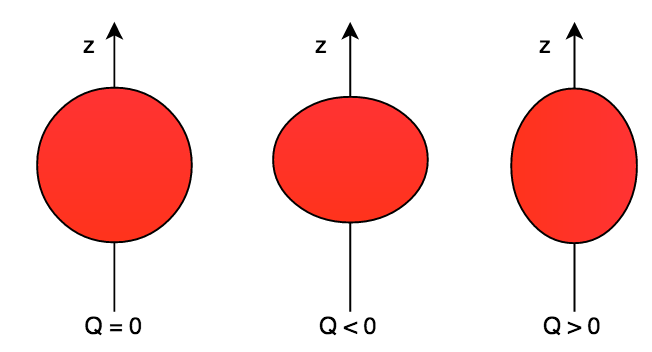
\includegraphics[width=\textwidth]{Graphics/Q_pic.png}
\caption[Oblate vs. Prolate vs. Spherical]{\small Shape of the nucleus for Q $=$ 0 (spherical), Q $<$ 0 (oblate) and Q $>$ 0 (prolate).\cite{wolf}}
\label{Q}
\end{center}
\end{figure}

In reality, direct measurement of Q is not feasible, as the nucleus is rotating. Instead, the spectroscopic quadrupole, Q$_s$, is measured. Q$_s$ is defined as the projection of Q onto the axis of quantization of the nucleus, and is given by
\begin{equation}
\mathrm{Q}_s = \frac{\mathrm{I}(2\mathrm{I}-1)}{(\mathrm{I}+1)(2\mathrm{I}+3)}\mathrm{Q},
\end{equation}
The use of $Q_s$ as a measure of $Q$ is valid under the assumption that the nuclear deformation is axially symmetric. Additionally, it is assumed that the axis of symmetry has a well defined direction with respect to \textbf{I}.

The Hamiltonian for the interaction between the spectroscopic electric quadrupole moment and the electric field produced by the electrons at the nucleus, $E_N$, is given by

\begin{equation}
\mathcal{H} = - \frac{1}{6}e\mathrm{Q}_s\nabla{E_N}
\end{equation}
where
\begin{equation}
\nabla{E_N} = \frac{\partial^2V}{\partial x_i\partial x_j}, \{x_j,x_k\} \in \{x,y,z\} \otimes \{x,y,z\},
\end{equation}
$e$ is the fundamental charge and $V$ is the electric potential. Recalling that the nuclear deformation is symmetric about the axis of quantization, the shift in energy is then given by

\begin{equation}
\Delta E_{\mathrm{Q_s}} = \frac{B}{4}\left[\frac{\frac{3}{2}K(K+1)-2\mathrm{I}(\mathrm{I}+1)\mathrm{J}(\mathrm{J}+1)}{\mathrm{I}(2\mathrm{I}-1)\mathrm{J}(2\mathrm{J}-1)}\right]
\label{B-eq}
\end{equation}
where $B$ is a hyperfine coefficient and is given by
\begin{equation}
B = e\mathrm{Q_s}\left\langle\frac{\partial^2V}{\partial z^2} \right\rangle
\end{equation}
Eq. \ref{B-eq} has singularities at I = $\frac{1}{2}$ and J=$\frac{1}{2}$. This captures the fact that in either case there is no coupling between the nucleus and the electric field gradient produced by the electrons, as an orbital angular momentum state of $\frac{1}{2}$ is isotropically distributed in space .

\subsubsection{The Hyperfine Equation}
The resonant energy of a transition between $\ket{g}=\ket{n_g,\mathrm{\textbf{F}_g=\textbf{I} + \textbf{J}_g}}$ and $\ket{e}=\ket{n_e,\mathrm{\textbf{F}_e=\textbf{I} + \textbf{J}_e}}$ is then given by
\begin{equation}
E_{hfs} = E_{fs} +  \Delta E_{\mathrm{A,A'}}+\Delta E_{\mu_I}\Bigr|_{\mathrm{F_g},I,J_g}^{\mathrm{F_e},I,J_e}+\Delta E_{\mathrm{Q_s}}\Bigr|_{\mathrm{F_g},I,J_g}^{\mathrm{F_e},I,J_e}.
\label{HFE}
\end{equation}

\noindent When a hyperfine spectrum is fitted, the fit parameters which govern the locations of the peaks are the hyperfine parameters $A$ and $B$ for both $\ket{e}$ and $\ket{g}$, as well as what is known as the centroid, $\nu_0$. The centroid combines the fine structure energy and the isotope shift into one quantity. It is important to note that while the values of hyperfine coefficients can be directly linked to the physical properties of the nucleus, only the change in the centroid with respect to a reference isotope can be used to measure the change in the mean-square charge radius.

\subsection{Peak intensities} 
The other notable characteristic of a hyperfine spectrum, the ratios of the peak intensities can give information as to the spin of the nucleus if the angular momentum states of the electron orbitals are known. The origin of the peak intensities is presented in more detail in the Angular Part of $\S$ \ref{ALI}, however in the interest of the completeness of this section, the result is presented here. The intensity of a transition from $\ket{\mathrm{F_e,J_e,I}}$ to $\ket{\mathrm{F_g,J_g,I}}$, relative to other available transitions, is known as the Racah intensity and is given by
\begin{equation}
Intensity = (2F_e+1)(2F_g+1)
\left\lbrace
\mathrm{
\begin{matrix}
\mathrm{F_g} & \mathrm{F_e} & 1\\
\mathrm{J_e} & \mathrm{J_g} & \mathrm{I} 
\end{matrix}
}
\right\rbrace^2
\label{RACAH}
\end{equation}
where the quantity in curly brackets is the Wigner 6-j symbol\cite{TomT}. An important property of the Racah intensities is the dependence on I. In cases where the value of I may be ambiguous, the relative intensities of the transitions can be used to discriminate between values of I.
\subsection{Peak Widths}
The lineshape of the peaks is the result of three physical processes, outlined in this section. These three processes are of varying importance, depending on the properties of the atoms being probed, contributing Lorentzian or Gaussian profiles to the peak shape. 

\noindent \subsubsection{Natural Linewidth}
\noindent The first addition to the linewidth of an atomic transition is the natural linewidth. The energy-time version of the uncertainty principal, $\Delta E \Delta t= \hbar$ leads to 
\begin{equation}
\Delta \nu = \frac{\Delta E}{h}=\frac{1}{2 \pi \tau_0}
\end{equation}
where $\tau_0$ is the mean lifetime of the state and $\Delta \nu$ is the full width half maximum of the Lorentzian profile describing the natural lineshape of an atomic transition\cite{TomT}.

\noindent \subsubsection{Power Broadening}
Stimulated emission occurs when an atom in an excited state is in the presence of photons with energy similar to an available atomic transition. In the case of laser spectroscopy, the laser provides the source of stimulating photons. Stimulated emission leads to power broadening, which depends on the power of the laser. The lifetime of a state will decrease according to
\begin{equation}
\frac{1}{\tau}= \frac{1}{\tau_0}\sqrt{1+\frac{I}{I_s}},
\end{equation}
where $I$ is the laser intensity and $I_s$ is the saturating laser intensity, which occurs when the rate of absorption is equal to the rate of stimulated emission on resonance. The expected lifetime of an excited electron decreases, resulting in a Lorentzian contribution to the lineshape as a consequence of the energy-time version of the uncertainty principal\cite{TomT}.
\subsubsection{Doppler Broadening}
Doppler broadening occurs when the atoms have a thermal velocity spread along the direction of propagation. This velocity spread leads to a shift in the frequency of the laser observed as by the atoms. The velocity distribution of a collection of atoms with mass $m_A$ at temperature $T$, along an axis $z$, is given by the so-called Maxwell-Boltzmann distribution \cite{thermal}
\begin{equation}
P(v_z) = \sqrt{\frac{m_A}{2 \pi kT}}\exp\left(-\frac{m_Av_z^2}{2kT}\right)
\label{MBD}
\end{equation}
\noindent where $k$ is the Boltzmann constant and $v_z$ is the velocity component of the atoms along the $z$-axis. The half width half maximum (HWHM) of this distribution is
\begin{equation}
\mathrm{HWHM} = \sqrt{\frac{2\log{(2)}kT}{m_A}}.
\end{equation}
For a Gaussian lineshape, the HWHM is also give by
\begin{equation}
\mathrm{HWHM} = \sqrt{2\log(2)}\sigma_g
\end{equation}
where $\sigma_g$ the square root of the variance of the distribution, $\sigma_g^2 = kT/m_a$ in the case of a Gaussian profile. When an observer is moving relative to a source of radiation, the frequency of the radiation measured by the observer obeys the following\cite{landau1975}
\begin{equation}
\nu_o = \nu_s\sqrt{\frac{1+v/c}{1-v/c}}
\label{dop_shift}
\end{equation}
where $\nu_o$ and $\nu_s$ are the observed and source frequencies, respectively, $v$ is the velocity of the observer relative to the source and $c$ is the speed of light in a vacuum. Differentiating the above with respect to $v$, and assuming $v\ll c$ leads to
\begin{align*}
\frac{d\nu_o}{dv} =& 2\frac{\nu_s}{c}\\ \nonumber
d\nu_o =& \nu_s\left(\frac{8kT\log(2)}{m_Ac^2}\right)^{1/2}
\end{align*}
\label{temp_width}
$d\nu_o$ is the HWHM of the Gaussian lineshape that Doppler broadening contributes to the overall lineshape of the transition\cite{TomT}.

\subsubsection{Voigt Profile}
As the strengths of the above processes can change depending on the parameters of the experiment, a Voigt profile is used when fitting the hyperfine spectra. The Voigt profile, defined as a convolution of the Lorentzian and Gaussian profiles, has no exact analytic solution. For the purposes of this work, the Pseudo-Voigt profile, given below, is used.
\begin{equation}
\mathcal{V}(x) = \frac{1-\epsilon}{\sigma_g\sqrt{2\pi}}\exp\left(\frac{(x-x_0)^2}{2\sigma_g^2}\right)+\frac{\epsilon\sigma}{\pi((x-x_0)^2+\sigma^2)}
\end{equation}
This is the weighted sum of a Gaussian and a Lorentzian where $\epsilon$ is a parameter that determines the relative contribution of the each and $x_0$ is the centroid. $\sigma$ is the Voigt linewidth and $\sigma_g = \sigma/\sqrt{2\log{2}}$ is defined such that the full width half maximum of the profile as well as its components is $2\sigma$.\cite{voigt}
\section{Spontaneous Emission in \\ Multi-Level Atoms}
\label{ALI}
A hyperfine spectrum is constructed through the measurement of the photons emitted as electrons in excited states de-excite to lower energy states. In order to simulate a hyperfine spectrum, then, it is necessary to understand the mechanisms through which electrons transition between energy levels in an atom.

Consider a two-level atom in an excited state. The wavefunction of the system is given by
\begin{equation}
\ket{\psi} = c_{e,0}e^{-i\omega_et}\ket{e,0} + \sum_Sc_{g,1}e^{-i(\omega_g+\omega)t}\ket{g,1_S}
\end{equation}
where $S = (\bm{k},\bm{\varepsilon})$ gives the wavevector $\bm{k}$ and polarization $\bm{\varepsilon}$ of an emitted photon, $\omega = kc$, $\omega_e$ and $\omega_g$ are the angular frequencies corresponding to the energy of the excited and ground states, respectively. \cite{LasCool} The time evolution of the two states is described by
\begin{align}
i\frac{\mathrm{d}c_{e,0}(t)}{\mathrm{d}t} =& \sum_Sc_{g,1_S}(t)\Omega_S e^{-i(\omega-\omega_a)t} \label{dc_e} \\
i\frac{\mathrm{d}c_{g,1_S}(t)}{\mathrm{d}t} =& \ c_{e,0}(t)\Omega_S^*e^{i(\omega-\omega_a)t} \label{dc_g}
\end{align}
where the coupling between each state is given by the Rabi frequency \\$\Omega_s = -\bm{\mu}\cdot\bm{E}_{\omega}/\hbar$. The electric dipole moment, $\bm{\mu}$ between two states is given by
\begin{equation}
\bm{\mu} = e\bra{e}\bm{r}\ket{g} 
\end{equation}
and the electric field per mode is given by
\begin{equation}
\bm{E}_{\omega} = \sqrt{\frac{\hbar\omega}{2\epsilon_0V}}\bm{\varepsilon}.
\end{equation}
$V$ is the volume over which the field is quantized and will eventually drop out. Integration of Eq. \ref{dc_g} and substitution of the result into Eq. \ref{dc_e}, followed by further integration yields 
\begin{equation}
\frac{d c_{e,0}(t)}{dt} = -\frac{\gamma}{2}c_{e,0}(t),
\end{equation}
where
\begin{equation}
\gamma = \frac{\omega^3\mu^2}{3\pi\epsilon_0\hbar c^3}
\label{gamma}
\end{equation}
is the decay rate for the population of the excited state, $\omega$ is the frequency of the transition and $c$ is the speed of light in a vacuum. The mean lifetime of the excited state is given by $\tau = 1/\gamma$. For an excited state where multiple decay paths are available, the total decay rate, $\gamma_t$ is given by
\begin{equation}
\frac{1}{\gamma_t} = \sum_i \frac{1}{\gamma_i}
\label{totdec}
\end{equation}
where the $\gamma_i$ are the partial decay rates for each decay path.


\subsection{The Dipole Moment}
In general, calculating the dipole moment  $\mu = \bra{e} \bm{\varepsilon} \cdot \bm{r} \ket{g}$ is not a simple task. 
In the simplest case (read hydrogenic wavefunctions), the Wigner-Eckart theorem states that the dipole moment can be split into two separate quantities in the following manner \citep{LasCool}
\begin{equation}
\mu_{eg} = e \mathcal{R}_{n_e J_e, n_g J_g}\mathcal{A}_{J_eJ_e^z, J_gJ_g^z}
\label{muref}
\end{equation}
where $\mathcal{R}_{n_e J_e, n_g J_g}$ and $\mathcal{A}_{J_eJ_e^z, J_gJ_g^z}$ are the radial and angular parts of the dipole moment, described in more detail below. 
\subsubsection*{Radial Part}
In most cases where the hyperfine structure is being probed, the radial part of the dipole moment only acts as an overall multiplicative factor for the strength of the coupling between the excited and ground states. This is due to the fact that all available ground states typically share the same radial wavefunction, likewise in the case of the excited states. The radial part is given by
\begin{equation}
\mathcal{R}_{n_e J_e, n_g J_g} = \bra{R_{n_e J_e}}\bm{r}\ket{R_{n_g J_g}} = \int_0^{\infty}r^2R_{n_e J_e}(r)rR_{n_g J_g}(r)dr
\end{equation}
where the $R_{nJ}$ are the hydrogenic radial wavefunctions of their respective states
\begin{equation}
R_{nJ}(r) = N_{nJ}\rho^J\exp(-\rho/2)J_{n-J-1}^{2J+1}(\rho)
\end{equation}
where $N_{nJ}$ is a normalization constant and $J_{n-J-1}^{2J+1}(\rho)$ are the Laguerre polynomials evaluated at $\rho = 2r/na_0$, where $a_0$ is the Bohr radius. The $J_{n-J-1}^{2J+1}(\rho)$ can be expanded in a power series
\begin{equation}
J_{n}^{m}(r) = \sum_{k=0}^{n} c_kr^k
\end{equation}

It is possible to extend this analysis to atomic structures that have an isolated electron sitting outside a closed shell. This is done using the effective principal quantum number $n^*= n - \delta_{J}$, where $\delta_{J}$ is called the quantum defect and depends on the orbital angular momentum \textbf{J}. This extended analysis is, however, not necessary, as an empirical measure of $ \mathcal{R}^2_{n_e J_e, n_g J_g}$ is easily obtained, and remains constant over all hyperfine transitions. This is done through the use of the decay rate of the fine-structure transition, $\gamma_f$. From Eq. \ref{totdec}, the decay rate of the fine-structure excited state is given by
\begin{equation}
\frac{1}{\gamma_f} = 3 \pi \epsilon_0 \hbar c^3 \sum_i \frac{1}{\omega_i^3 \mu_i^2}
\end{equation}
Substitution of Eq. \ref{muref} in to the above yields
\begin{equation}
\frac{1}{\gamma_f} = \frac{3 \pi \epsilon_0 \hbar c^3}{\mathcal{R}^2e^2} \sum_i \frac{1}{\omega_i^3\mathcal{A}^2_i}
\end{equation}
where the subscripts on $\mathcal{R}$ and $\mathcal{A}$ have been dropped for convenience. Rearranging gives the following expression for $\mathcal{R}^2$
\begin{equation}
\mathcal{R}^2 = \frac{3 \pi \epsilon_0 \hbar c^3 \gamma_f}{e^2} \sum_i \frac{1}{\omega_i^3\mathcal{A}^2_i}
\label{Remp}
\end{equation}
Note that this result allows $\mathcal{R}$ to take both negative and positive values. For the purposes of the calculations present in this work, however, only the square of the radial part is important. As such, the degeneracy in Eq. \ref{Remp} can safely be ignored. 
\subsubsection*{Angular Part}
Unlike the radial part of the dipole moment, the angular part changes depending on the F state of the excited and ground states. An outline of the procedure followed to find $\mathcal{A}$ is outlined in this section, a complete treatment of the calculation can be found in \cite{LasCool} 

In the presence of hyperfine structure, the atomic eigenstates can be represented in the following manner
\begin{equation}
\ket{n,F,F_z} = \sum_iC_i\ket{n,J,J_z}\ket{I,I_z}
\label{jstates}
\end{equation}
where \textbf{J}  =\textbf{ J} + \textbf{S}, \textbf{S} is the spin of the electron and the $C_i$'s are Clebsch-Gordan coefficients. The \textbf{J} states can further be decomposed into combinations of \textbf{J} and \textbf{S} states
\begin{equation}
\ket{n,F,F_z} = \sum_iC_i\ket{I,I_z}\sum_kC_k\ket{n,J,J_z}\ket{S,S_z}
\label{jstates}
\end{equation}
This is possible since the optical electric field only couples the orbital angular momentum, \textbf{J}, components of the eigenstates.  The Clebsch-Gordan coefficients can be expressed as
\begin{equation}
C_i = \braket{\mathrm{J,J_z ; S,S_z}|\mathrm{J,J_z}}=(-1)^{\mathrm{-J+S-J_z}}\sqrt{\mathrm{2J+1}}
\left(
\begin{matrix}
\mathrm{J}-\mathrm{S} & \mathrm{S} & \mathrm{J}\\
\mathrm{J}_z-\mathrm{S} & \mathrm{S}_z & -\mathrm{J}_z
\end{matrix}
\right)
\end{equation}
where the quantity in brackets is the Wigner 3-j symbol.
Substituting Eq. \ref{jstates} into the definition of $\mu$ gives 
\begin{equation}
\begin{split}
\mu = \sum_{q = -1,0,1} e (-1)^{\mathrm{1+J_e+J_g+I-F_{e,z}}}\mathcal{R}_{n_e J_e, n_g J_g}\\
\times \sqrt{(2J_g+1)(2J_e+1)(2F_g+1)(2F_e+1)}\\
\times \left\lbrace
\begin{matrix}
\mathrm{J}_e-\mathrm{S} & \mathrm{J}_e & \mathrm{S}\\
\mathrm{J}_g & \mathrm{L}_g-\mathrm{S} & 1
\end{matrix}
\right\rbrace
\left\lbrace
\begin{matrix}
\mathrm{J}_e & \mathrm{F}_e & \mathrm{I}\\
\mathrm{F} & \mathrm{J}_g &1
\end{matrix}
\right\rbrace
\left(
\begin{matrix}
\mathrm{F}_g & 1 & \mathrm{F}_e\\
\mathrm{F}_{g,z} & q &-\mathrm{F}_{e,z}
\end{matrix}
\right)
\end{split}
\end{equation}
where the quantity in the curly brackets is not a 3-j symbol but a 6-j symbol, and $q$ is the polarization of the electric field (1,0,-1). Recalling that $\mathcal{R}_{n_e J_e, n_g J_g}$ is a multiplying factor only and can be pulled out of the summation, then the angular part of $\mu$ (Eq. \ref{muref}) is given by
\begin{equation}
\begin{split}
\mathcal{A} = \sum_{q = -1,0,1} e (-1)^{\mathrm{1+J_e+J_g+I-F_{e,z}}}
\times \sqrt{(2J_g+1)(2J_e+1)(2F_g+1)(2F_e+1)}\\
\times \left\lbrace
\begin{matrix}
\mathrm{J}_e-\mathrm{S} & \mathrm{J}_e & \mathrm{S}\\
\mathrm{J}_g & \mathrm{J}_g-\mathrm{S}& 1
\end{matrix}
\right\rbrace
\left\lbrace
\begin{matrix}
\mathrm{J}_e & \mathrm{F}_e & \mathrm{I}\\
\mathrm{F} & \mathrm{J}_g &1
\end{matrix}
\right\rbrace
\left(
\begin{matrix}
\mathrm{F}_g & 1 & \mathrm{F}_e\\
\mathrm{F}_{g,z} & q &-\mathrm{F}_{e,z}
\end{matrix}
\right)
\end{split}.
\end{equation}


\subsection{Selection Rules}
The coupling of the ground state and excited state through the optical electrical field places restrictions on the change in the angular momentum state of the atom. In the case of transitions between orbital angular momentum states present in hyperfine atomic structures, only transitions where $\Delta$\textbf{F}  $=\pm1,0$ are permitted. These selection rules reflect conservation of angular momentum. Photons have angular momentum $\hbar$. The angular momentum of the photon can either be parallel, anti-parallel or perpendicular to the axis of quantization, reflecting $\Delta$\textbf{F}$=\pm1,0$ respectively. Additionally, the transition \textbf{F}' = 0 $\rightarrow$ \textbf{F} = 0 is forbidden. This is because \textbf{F} is a result of the coupling between \textbf{I} and \textbf{J}. \textbf{F}' = 0 implies that \textbf{I} = 0 = \textbf{J}'. The emission of a photon requires a change in angular momentum, which is impossible if \textbf{F} = 0 = \textbf{I} + \textbf{J}.

\section{Photon Scattering Rates}
The rate at which photons are absorbed by atoms is an important factor in the simulation of hyperfine spectra. For a two level system, where the population of the the excited state $\rho_{e}$ and the ground state $\rho_{g}$ obey the conservation rule $\rho_e +\rho_g = 1$, the total scattering rate from a laser field is given by
\begin{equation}
\gamma_p =  \frac{s_0/2}{1+s_0+(2\delta/\gamma)^2}
\label{scatt_rate}
\end{equation}
where $s_0$ is the on resonance saturation parameter $s_0 = I_l/I_s$, $\delta$ is the detuning parameter and $\gamma$ is the decay rate of the excited state. $I_l$ is the intensity of the laser field and $I_s$ is the saturation intensity defined as
\begin{equation}
I_s \equiv \frac{\pi h c}{3 \lambda^3 \tau}
\end{equation}
where $\lambda$ is the wavelength of emission of a resonant photon and $\tau = 1/\gamma$ is the lifetime of the excited state. The detuning parameter can be defined as
\begin{equation}
\delta =|f_{l} - f_{res}|
\end{equation}
where $f_l$ is the frequency of the laser and $f_{res}$ is the resonant frequency of the transition\cite{LasCool}. Eq. \ref{scatt_rate} provides an easy evaluation of the expected time for an on-resonance photon to be absorbed, which will be needed in the next chapter.

